\documentclass{article}\usepackage{graphicx}
\usepackage[a4paper, margin=1in]{geometry}
\usepackage{hyperref}
\usepackage{titlesec}
\usepackage{todonotes}

\titleformat{\section}{\large\bfseries}{}{0em}{}

\title{\textbf{Chat Vibe Check: Project Proposal}}
\begin{document}
\maketitle

\section{Project Metadata}
\begin{itemize}
    \item \textbf{Project Title:} Chat Vibe Check
    \item \textbf{Team Members Name:} 
    \begin{itemize}
        \item Deepa Rukmini Mahalingappa (34040788, drukminimaha@umass.edu)
        \item Benjamin Ibasco (28561432, bibasco@umass.edu)
        \item Javin Mendiratta (33328658, jmendiratta@umass.edu)
    \end{itemize}
   
    \item \textbf{Project Repository:} \href{https://github.com/bibascoumass/chat-vibe-check}{GitHub Repository Link}
\end{itemize}

\section*{Overview and Motivation}
Everyone chats. Everyone texts. But we don't all text the same- and the way we text can tell us a lot not only about ourselves, but also the people with whom we converse. Current chat visualization tools focus on the quantitative- how often you text, what times you text most often, who you text the most, and so on. But texting, and conversation in general, is inherently emotional and qualitative in nature. We wanted to design and create a platform that can analyze not only the quantitative, but also the qualitative. More specifically, our motivation is to build a website that can not only provide information on your chat/texting specifics, but also provide deeper insight into your interpersonal relationships and various sentiments across conversations. To give our analysis a focus and structure, we wanted to analyze chats based on the principles defined by modern psychological frameworks, such as attachment style and behavioral analysis.
\\\\
Some more specific goals include:
\begin{itemize}
    \item Comparing overall sentiment in a conversation (group and individual) over various time periods
    \item Analyzing sentiments expressed across various conversation topics to provide insight into individual/group perspectives 
    \item Displaying response times at various points in the day and for different topics
    \item Estimating behavioral tendencies and attachment style of chat members using the aforementioned metrics
\end{itemize}

\section*{Related Work}
The main inspiration of the project mainly came from the fact that there is growing empirical evidence that arranged marriages are scoring better on metrics like satisfaction and divorce rates compared to traditional marriages (\href{https://www.psychologytoday.com/us/blog/the-science-behind-behavior/201511/why-are-so-many-indian-arranged-marriages-successful}{PyschologyToday.com article}). At the time, we were interested in exploring the reasons why and quickly realized this would be a challenging goal . We then explored narrowing the scope but staying on the theme of understanding relationships and was inspired by personal chat visualizations done by users analyzing trends in their relationship (\href{https://github.com/bibascoumass/chat-vibe-check}{Example from Reddit}). From the examples we noticed the visualizations or insights were very surface level and thought that there might be use for a tool that tried to explore more meaningful behavioral patterns from the chat data. To get a better direction on how or what we would try to observe from the chat data, we decided to base our analysis around an actual psychological framework and we chose Attachment Theory for this.  

\section*{Questions}
The main question we're trying to answer is what behavioral patterns can we observe from chat message interactions between people two get a better understanding of their attachment styles? As we explored this idea, we focused on two key derived attributes: Sentiment and engagement. From this realization we focused on having our visualizations answer the following questions:
\begin{itemize}
    \item How does the sentiment of my conversation evolve over time?
    \item Are there certain conversation topics that are intensly positve or negative? 
    \item Are there periods of time or topics in my conversation when a person is less responsive than usual or tries to avoid or change the topic? 
\end{itemize}

\section*{Data}
To prototype the data pre-processing and ingestion implementations, we decided to just work with our own Whatsapp group chat data as we just needed to work with the data format for the messaging platform we wanted to support. 
\\\\ To prototype the visualizations, it was difficult to find a WhatsApp chat dataset in English so we settled on using a dataset from Kaggle of over one million two-person chat logs related to Ubuntu technical support: https://www.kaggle.com/datasets/rtatman/ubuntu-dialogue-corpus/data . At this early stage, there hasn't been a need to do any pre-processing on this dataset. 
\\\\ The following datasets were also considered:
\begin{itemize}
    \item \href{https://github.com/dhfbk/WhatsApp-Dataset}{Movie Dialogue Corpus} - Initially chosen as a backup in the worst case scenario wherein we couldn't find two person conversation chat data in English. 
    \item The following WhatsApp chat datasets were considered and although there are analysis libararies that support multiple languages (e.g. multilang-sentiment) we ultimately avoided these as we wouldn't be able to compare the results of our analysis to what we thought the data was actually expressing. 
    \begin{itemize}
        \item \href{https://www.kaggle.com/datasets/Cornell-University/movie-dialog-corpus/data}{WhatsApp Chat used for studying cyberbullying in Italy}
        \item \href{https://www.kaggle.com/datasets/mmuhammetcavus/whatsapp-chat/data}{WhatsApp Group Chat in Hindi}
    \end{itemize}
\end{itemize}

\section*{Exploratory Data Analysis}
\begin{itemize}
    \item \textbf{Download:} We'll need to make sure that our website references instructions on how to download the data from our supported platforms.
    \item \textbf{Cleanup:} We'll need to ingest data from multiple formats and store it such that we can at least query for the message itself and the following metadata: sender, receiver, send time, seen time (this may not be available on all platforms).
    \item \textbf{Quantities:} The quantities we expect to derive from the data are sentiment, response time, engagement, and conflict resolution metrics relative to topics and time.
    \item \textbf{Analysis:} We've decided for now that we'll keep the scope simple in the beginning and only focus on text messages and emojis. Video, audio, GIFs, and images will be ignored in the onset.
\end{itemize}

\section*{Design Evolution}
The project aimed to extract and visualize emotional patterns from chat data in a way that is easy to interpret, interactive, and actionable. Our design evolved significantly from the initial proposal as we explored more effective ways to represent time-based and user-based sentiment trends.

\begin{itemize}
    \item \textbf{Initial Visualizations Considered:}
    \begin{itemize}
        \item Bar charts to show average sentiment per user or per day.
        \item Line charts for sentiment flow over time.
        \item Pie charts to show distribution of sentiment types.
        \item Snakey Diagram showing the flow of conversation state transitions from neutral to conflict to resolution.
    \end{itemize}

    \item \textbf{Final Visualizations Used:}
    \begin{itemize}
        \item \textbf{Heatmap:} Showcased sentiment variation across time periods (e.g., hourly/daily), helping identify emotional peaks.
        \item \textbf{Scatter Plot - Response Time vs Sentiment:} Revealed correlation between emotional intensity and reply latency.
        \item \textbf{Scatter Plot - Timestamp vs Sentiment:} Illustrated sentiment flow throughout the conversation, supporting detection of escalating or resolving emotional trends.
        \item \textbf{Chat Parser Table:} Provided a clean, searchable layout of individual messages with timestamps, user labels, and sentiment tags.
    \end{itemize}    

    \item \textbf{Deviations from Original Proposal:}
    \begin{itemize}
        \item Initially proposed line charts were replaced by scatter plots, which better captured the irregular and message-level nature of chat data.
        \item We're currently playing around relating time, topic and sentiment instead all in one chart rather than having a two separate ones for topic and then for time.
        \item The most basic implementation for showing the chat is currently just having it as a separate page but we will look into the displaying it as the user clicks on messages. 
    \end{itemize}
\end{itemize}
 \section*{Visualizations Used}

\begin{itemize}
    \item \textbf{Heatmap: Sentiment vs Time}
    \begin{itemize}
        \item \textbf{Design Goal:} To identify how sentiment changes over time (across hours or days), highlighting peak emotional periods like high negativity during specific hours.
        \item \textbf{Color Mapping:}
        \begin{itemize}
            \item \textcolor{red}{Red} = Negative
            \item \textcolor{green}{Green} = Positive
            \item \textcolor{gray}{Gray} = Neutral
        \end{itemize}
    \end{itemize}
    
    \item \textbf{Scatter Plot: Response Time vs Sentiment}
    \begin{itemize}
        \item \textbf{Design Goal:} To explore whether the speed of replies correlates with emotional tone, revealing patterns like faster responses during emotional conversations.
        \item \textbf{Design Enhancements:}
        \begin{itemize}
            \item Color-coded sentiment points for clarity.
            \item Tooltips on hover for detailed insights.
            \item Filter options by user or time range.
        \end{itemize}
        \item \textbf{Design Principles Used:}
        \begin{itemize}
            \item Data-ink ratio for clean visualization.
            \item Pre-attentive processing with color and shape to distinguish sentiment.
        \end{itemize}
    \end{itemize}
    
    \item \textbf{Scatter Plot: Timestamp vs Sentiment}
    \begin{itemize}
        \item \textbf{Design Goal:} To display sentiment flow chronologically over the chat session, allowing trend detection like escalating negativity or emotional recovery.
        \item \textbf{Design Decisions:}
        \begin{itemize}
            \item Smooth timeline across X-axis.
            \item Hover details with sentiment classification.
        \end{itemize}
        \item \textbf{Design Principle Used:}
        \begin{itemize}
            \item Temporal alignment of visual elements for easy scanning.
            \item Consistent color scale to maintain cognitive ease.
        \end{itemize}
    \end{itemize}
    
    \item \textbf{Chat Parser with Sentiment Tags}
    \begin{itemize}
        \item \textbf{Design Goal:} To convert raw chat into a clean, readable, and searchable table with labeled sentiment.
        \item \textbf{Features:}
        \begin{itemize}
            \item Each message row includes: Timestamp, User, Message, and Sentiment Score (with tag).
            \item Sentiment tags are color-coded.
            \item Optional search/filter by user or sentiment type.
        \end{itemize}
        \item \textbf{Design Principles Used:}
        \begin{itemize}
            \item Clarity and hierarchy through formatting, spacing, and alignment.
            \item Redundancy principle — sentiment shown via both text and color for accessibility.
        \end{itemize}

        
    \end{itemize}
\end{itemize}



\section*{Implementation}
Our implementation, at the current stage, features a home page for uploading documents, and 4 main features across 3 sub-pages. We plan to add more implementations, interactivity, and design consistency before out final submission.
\\\\
Before any of the views can be made, the user must upload their chat log to the website in order for it to be analyzed and parsed on the backend. As of now, our inputs must be a csv with the following format: (!). However, we plan to extend the input types to a more generic implementation.
\begin{itemize}
    \item Home page: This is the page where the user will select the file and upload it. After uploading the file, they can then choose a view from the toolbar. We will decide on and create a default view to show the user immediately upon upload to ensure a smoother and more natural experience. 
    \item 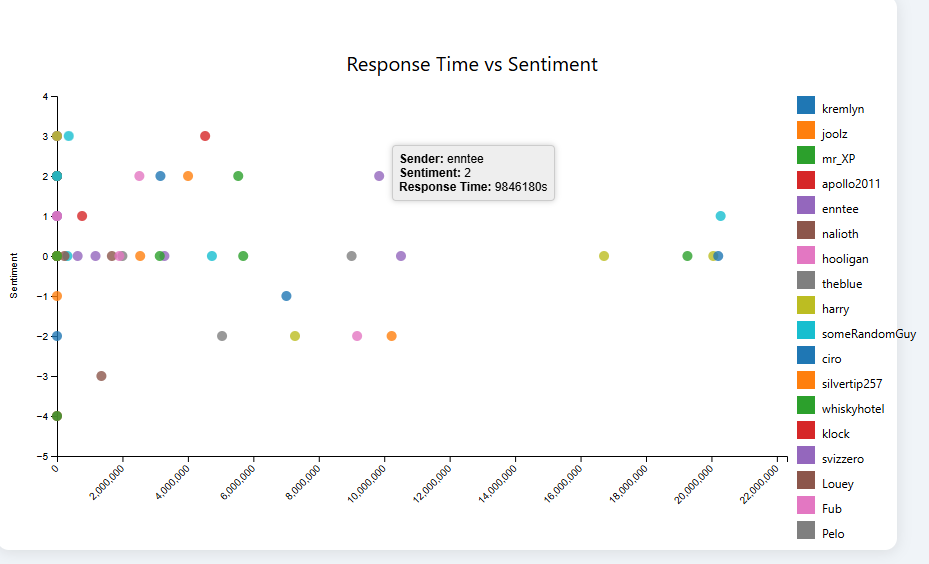
\includegraphics[width=10cm]{./Latex Images/Responsetime timeline ss.png}
    \item Time (X-axis) vs Sentiment (Y-axis) Scatterplot: Each point represents a message and each point is labeled by user. This plot is meant to showcase the various sentiments shown in the conversation over time, with colors of nodes corresponding to the users and the y-axis showing sentiment (positive vs negative). Each node (message) also displays the sender, sentiment, and timestamp when hovered over. Currently, the graph looks a little cluttered and is working for group messages. We want to see how it will look for smaller chats eventually and add a feature to specify members for group chats.
    \item 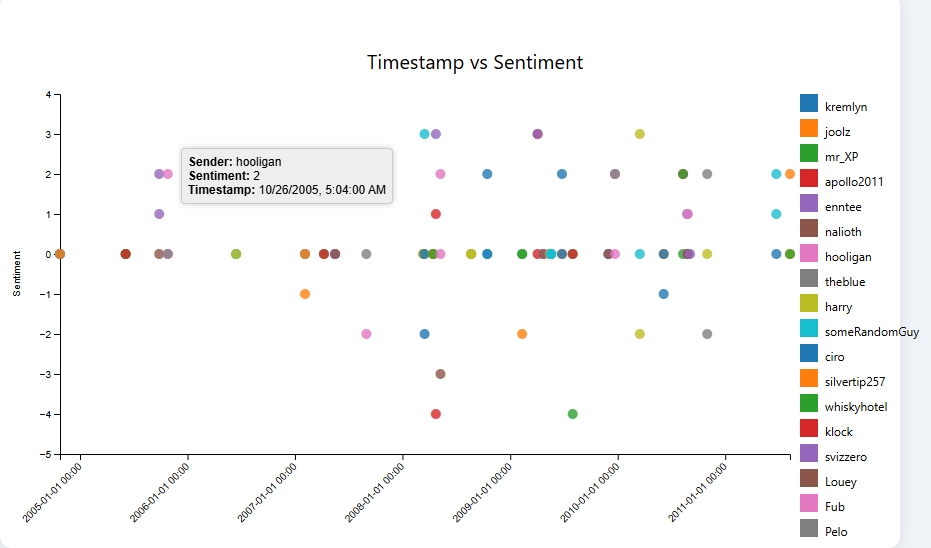
\includegraphics[width=10cm]{./Latex Images/Timeline Sentiment ss.png}
    \item Response Time (X-axis) vs Sentiment (Y-axis) Scatter Plot: Each point represents a message and each point is labeled by user. This plot is meant to showcase the various response times shown in the conversation for varying sentiments, with colors of nodes corresponding to the users and the y-axis showing sentiment (positive vs negative). Each node (message) also displays the sender, sentiment, and response time when hovered over. Currently, the graph is a little confusing to properly interpret. We are considering switching the axis to make response time the dependent variable, so we can analyze if different sentiments influence response time. We may expand this to include topic instead of sentiment as an axis, and explore different chart styles.
    \item 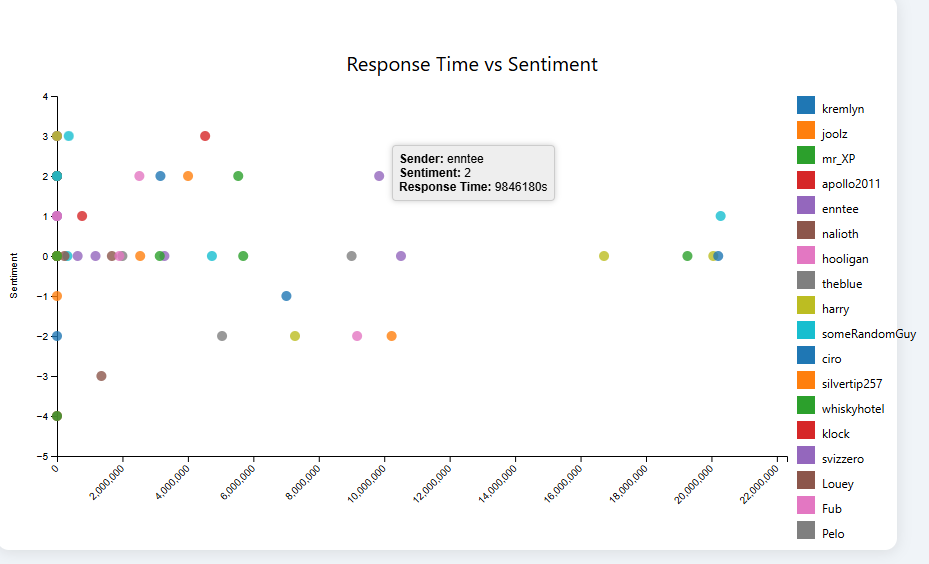
\includegraphics[width=10cm]{./Latex Images/Responsetime timeline ss.png}
    \item NEEDS WORK: Topic (X-axis) vs Sentiment (Y-axis) Heatmap: This graph is incorrect at the moment, as we need to update it. Currently we have the x-axis showing the timestamp of the message and the y-axis being discrete with certain topics. As such, a different chart style, where topics are more distinctly serrated may be in order. Additionally, our code that determines topics is somewhat faulty, and we need to broaden our range of topics to identity- right now every conversation is being placed in the "other" category. 
    \item 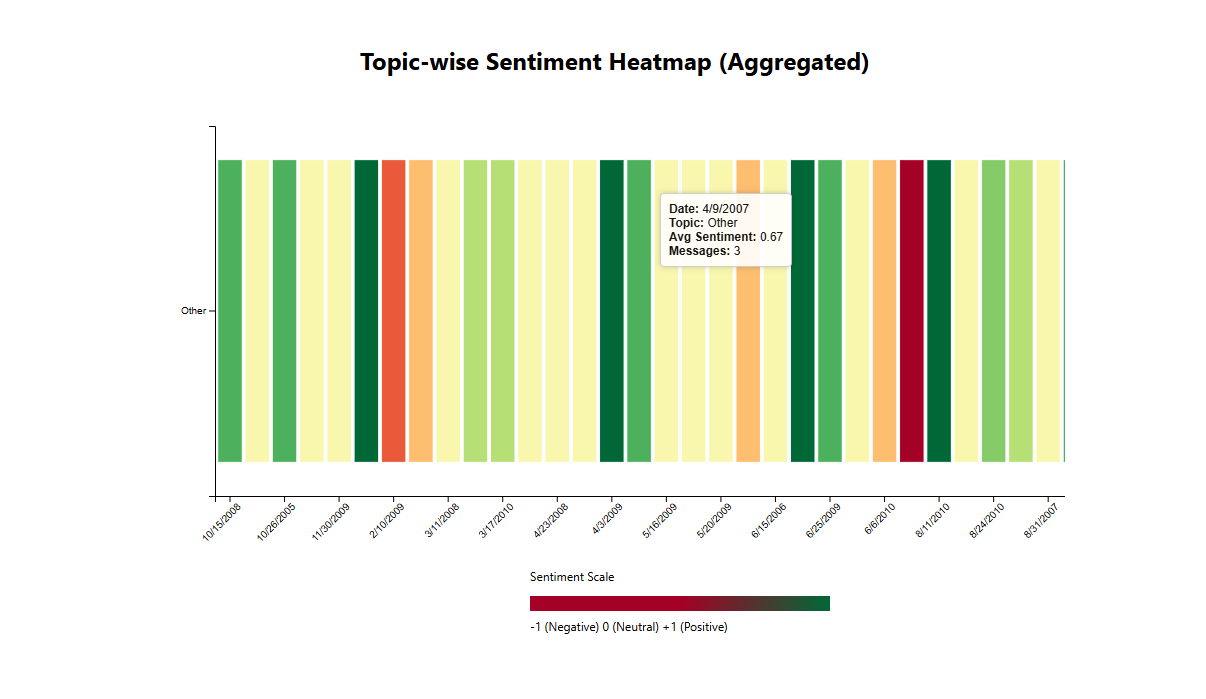
\includegraphics[width=10cm]{./Latex Images/Sentiment heatmap ss.png}
    \item Conversation Display: This visual simply lists out the entire chat conversation in a scroll-able text box, showing the message and it's corresponding sentiment. This is to provide a familiar interface to the user, while providing a more "overall" view of the data. We will need to incorporate pages or some effective way to split up the conversation for larger datasets.
    \item 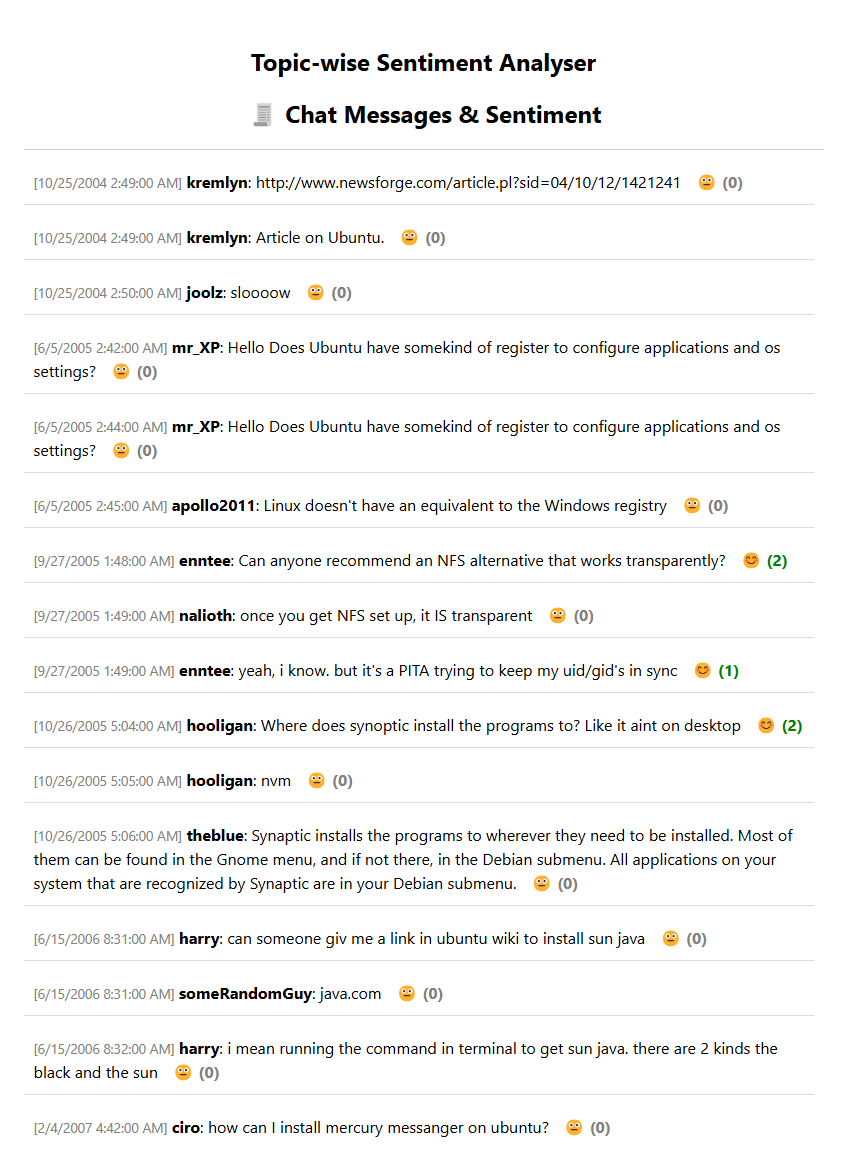
\includegraphics[width=10cm]{./Latex Images/Chat log ss.png}
\end{itemize}

\section*{Optional Features}
\begin{itemize}
    \item Message Grouping: We’ll need to decide if we’ll try to group messages together as part of the same conversation.
        \begin{itemize}
            \item We can base this off two criteria: topic and time. Starting with time-based grouping and then later by topic if time permitting.
        \end{itemize}
    \item Conflict Resolution Snakey Diagram: Depicting the flow of conversation state transitions from neutral to conflict to resolution.
    \item Give an attachment style assessment with a confidence score.
    \item Show each user's perceived attachment style over time.
    \item Show patterns of behavior based on sentiment and attachment style analysis relative to time and topics.
\end{itemize}
(Note: We’ve decided to make visualizations that try to use a derived attachment style metric optional, as we currently have no guarantee if the derived attributes conclusively determine attachment style.)

\section*{Security}
\begin{itemize}
    \item Client-side processing such that our data consists only of the messages, the timestamps and a generic username assigned like "User A" or "User B".
    \item Use our chosen hosting platform's (like Heroku) built-in HTTPS.
    \item Then we always want to delete the data once the user who has uploaded ends their session, so we're planning on using an in-memory datastore (like Redis) configured with TLS and disable any of its features that write the data to disk (like backups). This way we avoid needing to encrypt data on disk.
\end{itemize}

\section*{Tech Stack}
\begin{itemize}
    \item Front End: React, D3, Modal overlay library (react-modal?)
    \item Back End: Node.js + Express.js (Express for data ingestion REST APIs), Redis, some NLP library
    \item Deployment: Heroku, GitHub
\end{itemize}

\section*{Evaluation}
\begin{itemize}
    \item For such a project that asks users to require them to upload potentially sensitive data, the tool for sanitizing and removing that data needs to be within their control and trust. This was the main reason why we weren't able to initially get data from real people within our networks. 
    \item We still need to fix how we're identifying topics as the current implementation is finding it hard to identify specific topics in the content and just labeling a lot of data as "Other"
    \item Admittedly, we may have spent too much time expirmenting with applying the visualizations even in group settings and trying to group messages by topic/conversation so we still need to finetune the scatter plot visualization as well in terms of scoping the data to specific conversations to have more meaningful insights. 
\end{itemize}


\end{document}
